\documentclass[12pt]{article}
\usepackage[a4paper, margin=.30in]{geometry}
\usepackage{graphicx ,
            wrapfig,
            xcolor, 
            enumerate,
            amsmath,
            comment
            }

\newcommand\headerMe[2]{\noindent{}#1\hfill#2}
\renewcommand{\thesection}{\Roman{section}}


\begin{document}
% headers --------------
\headerMe{Matière : Physique-Chimie}{Professeur : Zakaria HAOUZAN}\\
\headerMe{Unité : Mesure en chimie}{Établissement : Lycée SKHOR qualifiant}\\
\headerMe{Niveau : 1BAC S-SM}{Heure : 7H}\\

% ------Content ________
\begin{center}

    \Large{Leçon N8: \color{red} Mesure de la conductance }

\end{center}

\section{Introduction}
    \subsection{Expérience : }
%\begin{wrapfigure}{r}{0.25\textwidth}
 %   \centering
On réalise le montage suivant : 
    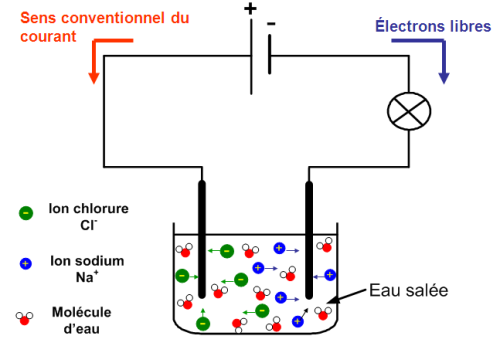
\includegraphics[width=0.25\textwidth]{./img/img00.png}
%\end{wrapfigure} 

\subsection{Observations: }
Lorsqu’on ferme l’interrupteur on constate que :
- les cations $Cu^{2+}$ caractérisés par la couleur bleue migrent vers la cathode (borne négative du générateur).

- les anions $MnO_4^-$ caractérisés par la couleur violette migrent vers l’anode (borne positive du générateur).

\subsection{Conclusion: }
Dans les solutions aqueuses, le passage du courant électrique est dû à un déplacement d’ions :
Les ions positifs se déplacent dans le sens conventionnel du courant (vers la borne - du générateur) et les ions négatifs dans
le sens contraire (vers la borne + du générateur).

\section{Conductance d’une solution ionique :G }
\subsection{la cellule conductimétrique: }
Pour déterminer la conductance d’une solution ionique on utilise la cellule conductimétrique .

Une cellule de conductimétrie est constituée de deux électrodes, de plaques identiques et parallèles
On plonge les plaques dans la solution électrolytique et on applique entre ses bornes une tension alternative sinusoïdale à l’aide d’un générateur basse fréquence GBF 

(pour éviter le phénomène d’électrolyse et afin que les mesures ne soient
pas perturbées par des réactions d’électrolyse).


    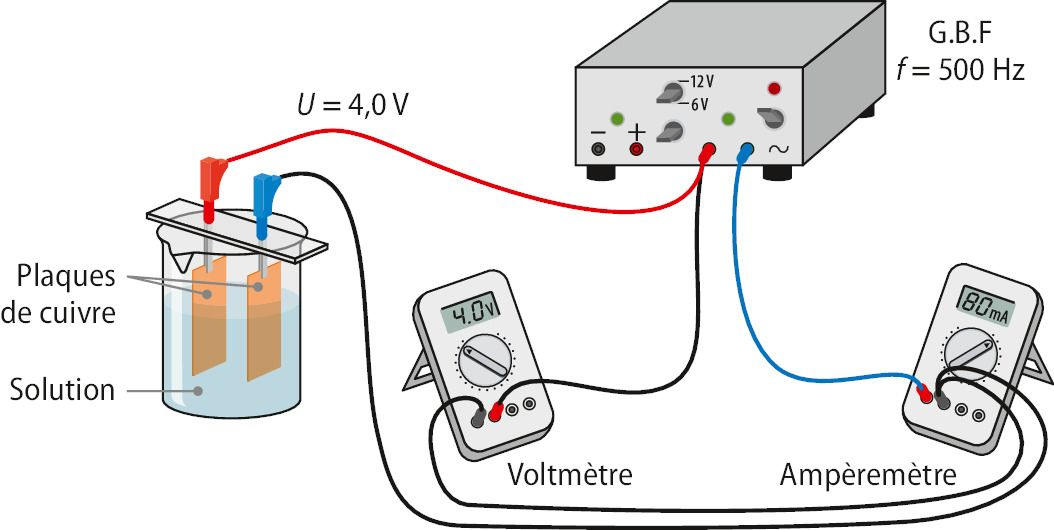
\includegraphics[width=0.4\textwidth]{./img/img01.jpg}

Pour mesurer la conductance G d'une solution électrolytique il suffit de mesurer la tension U entre les plaques de la cellule (plongées dans la solution ) et l'intensité I du courant qui traverse la solution.

La portion de la solution qui se trouve entre les deux plaque se comporte comme un dipôle de résistance $R = \frac{U}{I}$ et sa conductance $G = \frac{1}{R} = \frac{I}{U}$ en siemens S

\subsection{la conductance : }
La conductance d'une solution exprime son aptitude à conduire le courant électrique, elle est égale à l’inverse de la
résistance : $G = \frac{1}{R}$ R en $\Omega$ et G en siemens

\subsection{Mesure de la conductance : }
\begin{wrapfigure}[10]{r}{0.32\textwidth}

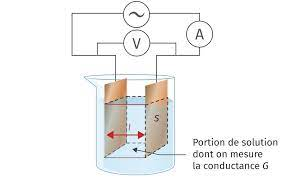
\includegraphics[width=0.30\textwidth]{./img/img02.jpeg}

\end{wrapfigure}
\subsubsection{Expérience 1 : Influence de la surface ,la distance entre les plaques}

Utilisons une solution de chlorure de sodium de concentration molaire c=$5.10^{-3}$ mol/L et effectuons les mesure suivante à
l’aide de la cellule conductimétrique

Cette expérience montre que conductivité dépend de la distance entre les deux plaques de la cellule conductimétrique et
de la concentration de la solution ainsi que de la surface en regard des deux plaques.

(pour varier la surface, il suffit de faire sortir partiellement les plaques de la solution) et (pour faire varier la concentration
, il suffit de réaliser soit la dilution de solution précédente en ajoutant de l’eau ou bien ajouter un peu de sel ).
Indiquons les résultats obtenus :

-Lorsque L augmente, G augmente.

-Lorsque S augmente , G diminue.

-Lorsque c augmente , G augmente.

\subsubsection{Expérience 2 : Influence des concentrations des espèces présents dans la solution :}

On prépare une solution de chlorure de sodium et une solution d’hydroxyde de sodium ayant même concentration.

La solution de chlorure de sodium de concentration c= 5.10-3mol/L (On l’obtient en dissolvant 146mg de sel de cuisine
dans 0,5L d’eau).$\rightarrow$ $Na^+$ et $Cl^-$

La solution d’hydroxyde de sodium de concentration c= 5.10-3mol/L (On l’obtient en dissolvant 100mg de sel de cuisine
dans 0,5L d’eau). $Na^+$ et $OH^-$

Pour chaque solution on mesure la conductivité.

L’expérience montre que la conductivité de la solution d’hydroxyde de sodium est plus grande que celle du chlorure de sodium malgré que les deux solutions ont même concentration.

Donc la conductance G dépend de des espèces chimiques ioniques présentes dans la solution.

\subsection{Facteurs influençant la conductance : }

La conductance G dépend de la nature de la solution. Pour une solution donnée, la conductance augmente quand :
\\- La surface S d’une électrode augmente ;
\\- la distance L entre les électrodes diminue ;
\\- la température $\theta$ de la solution augmente ;
\\- la concentration C de la solution augmente (G est proportionnelle à C).

\subsection{Courbe d’étalonnage : }
\begin{wrapfigure}{r}{0.2\textwidth}

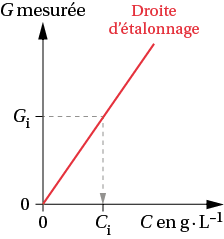
\includegraphics[width=0.20\textwidth]{./img/img03.png}

\end{wrapfigure}

On réalise une série de mesures de conductance pour des
solutions de concentrations connues afin de tracer la courbe
d'évolution de cette conductance en fonction de la
concentration.

La conductance varie en fonction de la concentration suivant
la loi de Kohlraush: G=K.C

Cette courbe d'étalonnage permet ensuite de retrouver la concentration inconnue de la solution à partir de la mesure de la conductance

\textbf{Les limites de cette méthode :} La méthode d’étalonnage conductimétrique à ses limites, en l’occurrence elle n’est pas applicable lorsque la solution est un mélange de plusieurs espèces ioniques (par exemple de l’eau de mer qui contient énormément d’ions différents en solution).  Pour des solutions peu concentrées $(C < 10^{-2} mol.L^{-1} )$

on constate que la conductance G d’une solution est proportionnelle à sa concentration C.

\section{ Conductivité d’une solution ionique : $\sigma$}
\subsection{Définition de la conductivité : }
La conductivité $\sigma$ représente l’aptitude d’une solution à conduire le courant électrique.

La conductance d’une solution est proportionnelle au rapport S/L; on écrit : $G=\sigma.\frac{S}{L}$

- $\sigma$ est la conductivité de la solution en $S.m^{-1}$ ;
\\- S est la surface des électrodes en $m^2$ ;
\\- L est la distance entre les plaques en $m$.
\\- S/L est appelé constante de cellule en $m$.

\subsection{Conductivité molaire ionique d’un ion :}
La conductivité d’un ion $X_i$ est proportionnelle à sa concentration : $$\sigma = \lambda_i . [X_i]$$

Le coefficient de proportionnalité $\lambda_i$ est appelé conductivité molaire ionique son unité est le   $S.m^2.mol^{-1}$

La conductivité molaire ionique dépend de la température, de la nature du solvant et de l’ion considéré.

\vspace{0.2cm}

Exemple : 

-pour l’ion hydroxyde  $OH^-$ , la conductivité molaire ionique à $25^oC$ est :$\lambda_i(H_3O^+)= 35 mSm^2/mol. $


-pour l’ion oxonium $H_3O^+$ , la conductivité molaire ionique à $25^oC$ est :$\lambda_i(OH^-)= 20 mSm^2/mol. $


\subsection{ Conductivité d’une solution : }
La conductivité d’une solution est notée $\sigma$. Elle dépend de chaque ion en solution.
Chaque ion possède une conductivité molaire ionique est notée $\lambda$.

La conductivité s de la solution est égale à la somme des conductivités due aux cations et aux anions. On
écrit : $\sigma = \sigma_i(cations) + \sigma_i(anions) $

$$\sigma = \sum \lambda_i.[X_i] = \lambda_1.[X_1] + \lambda_2.[X_2] + \lambda_3.[X_3] .....$$

Avec $\sigma$ en $S.m^-1$ ; $\lambda$ en $S.m^2.mol^{-1}$ et [Xi] en $mol.m^{-3}$ (attention à l’unité !)

\subsection{Conductivité molaire ionique de quelques ions : }
Tableau de valeurs des conductivités molaires ioniques limites tabulées de quelques ions à 298 K en solution
aqueuse :

\begin{center}
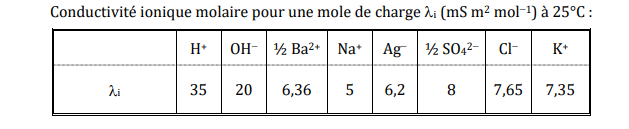
\includegraphics[width=0.8\textwidth]{./img/img04.png}
\end{center}

Les ions $H_3O+$ $(H^+_{(aq)})$ et $HO^-$ ont une conductivité molaire ionique nettement plus grande que celle des autres
ions, donc leur présence dans une solution confère à celle-ci une conductivité importante.


\end{document}
